\documentclass[11pt,a4paper]{article}
\pdfoutput=1
\usepackage{jinstpub}

%\usepackage{draftwatermark}

\newcommand{\ignore}[1]{}
%\renewcommand*\contentsname{Table of Contents}
\newcommand\todo[1]{}
\newcommand\stub[1]{\input{#1}}

% side-by-side figures
\usepackage{caption}
\usepackage{subcaption}

%%% Needed to make subsubsubsubsections...
\usepackage{titlesec}
\usepackage{multirow}
\usepackage{booktabs}
\usepackage{bm}
\usepackage{fancyhdr}
\usepackage{color}

\pagestyle{fancy}
%%% How deep do we count in ``sub''sections...
\setcounter{secnumdepth}{4}
%%% These lines do the re-purposing of paragraph into ``subsubsubsubsection''
\titleformat{\paragraph}
{\normalfont\normalsize\bfseries}{\theparagraph}{1em}{}
\titlespacing*{\paragraph}
{0pt}{3.25ex plus 1ex minus .2ex}{1.5ex plus .2ex}

%\renewcommand{\baselinestretch}{0.965}

% Some neutrino physics shortcuts
\newcommand{\nua}{\ensuremath{\nu_\alpha}\xspace}
\newcommand{\nub}{\ensuremath{\nu_\beta}\xspace}
\newcommand{\nue}{\ensuremath{\nu_e}\xspace}
\newcommand{\num}{\ensuremath{\nu_{\mu}}\xspace}
\newcommand{\nut}{\ensuremath{\nu_{\tau}}\xspace}
\newcommand{\nuabar}{\ensuremath{\bar{\nu}_\alpha}\xspace}
\newcommand{\nubbar}{\ensuremath{\bar{\nu}_\beta}\xspace}
\newcommand{\nuebar}{\ensuremath{\bar{\nu}_e}\xspace}
\newcommand{\numbar}{\ensuremath{\bar{\nu}_{\mu}}\xspace}
\newcommand{\nutbar}{\ensuremath{\bar{\nu}_{\tau}}\xspace}

\title{Deep Learning in Liquid argon time projection chambers: Optimizing the Architecture for Particle Classification}
\collaboration{MicroBooNE Collaboration}

\abstract{
Liquid argon time projection chambers (LArTPCs) produce image-like data that may be analyzed with deep neural networks (Deep Learning, or DL). This approach to data analysis is becoming more common in LArTPCs, as well as other high channel-count segmented detectors where the events leave imprints on the detector that may be interpreted as images. In particular, MicroBooNE is an 8256 wire detector viewing 89 tons fiducial liquid argon where DL studies have been performed~\cite{uB-JINST} and show great promise. That study showed progress in single particle classification as well as progress toward neutrino identification, using networks that were not necessarily chosen to be optimal. This paper reports results on single particle classification using DL network architectures in which the literature or experience suggest further progress can be made on images such as ours. We answer key questions about performance  on this problem as a function of network architectures and show that networks \_\_, \_\_ and \_\_ give functionally equivalent high performance, with gains in network \_\_ in resource consumption that suggest its use.
}

\begin{document}
% Authors in alphabetical order
\author[g]{R.~Acciarri}
\author[z]{C.~Adams}
\author[h]{R.~An}
\author[w]{J.~Asaadi}
\author[a]{M.~Auger}
\author[g]{L.~Bagby}
\author[g]{B.~Baller}
\author[q]{G.~Barr}
\author[q]{M.~Bass}
\author[x]{F.~Bay}
\author[b]{M.~Bishai}
\author[j]{A.~Blake}
\author[i]{T.~Bolton}
\author[m]{L.~Bugel}
\author[f]{L.~Camilleri}
\author[f]{D.~Caratelli}
\author[g]{B.~Carls}
\author[g]{R.~Castillo~Fernandez}
\author[g]{F.~Cavanna}
\author[b]{H.~Chen}
\author[r]{E.~Church}
\author[l,f]{D.~Cianci}
\author[m]{G.~H.~Collin}
\author[m]{J.~M.~Conrad}
\author[u]{M.~Convery}
\author[f]{J.~I.~Crespo-Anad\'{o}n}
\author[q]{M.~Del~Tutto}
\author[j]{D.~Devitt}
\author[s]{S.~Dytman}
\author[u]{B.~Eberly}
\author[a]{A.~Ereditato}
\author[c]{L.~Escudero Sanchez}
\author[v]{J.~Esquivel}
\author[z]{B.~T.~Fleming}
\author[d]{W.~Foreman}
\author[l]{A.~P.~Furmanski}
\author[k]{G.~T.~Garvey}
\author[f]{V.~Genty}
\author[a]{D.~Goeldi}
\author[i]{S.~Gollapinni}
\author[s]{N.~Graf}
\author[z]{E.~Gramellini}
\author[g]{H.~Greenlee}
\author[e]{R.~Grosso}
\author[q]{R.~Guenette}
\author[z]{A.~Hackenburg}
\author[v]{P.~Hamilton}
\author[m]{O.~Hen}
\author[l]{J.~Hewes}
\author[l]{C.~Hill}
\author[d]{J.~Ho}
\author[i]{G.~Horton-Smith}
\author[g]{C.~James}
\author[c]{J.~Jan~de~Vries}
\author[y]{C.-M.~Jen}
\author[s]{L.~Jiang}
\author[e]{R.~A.~Johnson}
\author[m]{B.~J.~P.~Jones}
\author[b]{J.~Joshi}
\author[g]{H.~Jostlein}
\author[f]{D.~Kaleko}
\author[l,f]{G.~Karagiorgi}
\author[g]{W.~Ketchum}
\author[b]{B.~Kirby}
\author[g]{M.~Kirby}
\author[g]{T.~Kobilarcik}
\author[a]{I.~Kreslo}
\author[q]{A.~Laube}
\author[b]{Y.~Li}
\author[j]{A.~Lister}
\author[h]{B.~R.~Littlejohn}
\author[g]{S.~Lockwitz}
\author[a]{D.~Lorca}
\author[k]{W.~C.~Louis}
\author[a]{M.~Luethi}
\author[g]{B.~Lundberg}
\author[z]{X.~Luo}
\author[g]{A.~Marchionni}
\author[y]{C.~Mariani}
\author[c]{J.~Marshall}
\author[h]{D.~A.~Martinez~Caicedo}
\author[i]{V.~Meddage}
\author[o]{T.~Miceli}
\author[k]{G.~B.~Mills}
\author[m]{J.~Moon}
\author[b]{M.~Mooney}
\author[g]{C.~D.~Moore}
\author[n]{J.~Mousseau}
\author[l]{R.~Murrells}
\author[s]{D.~Naples}
\author[t]{P.~Nienaber}
\author[j]{J.~Nowak}
\author[g]{O.~Palamara}
\author[s]{V.~Paolone}
\author[o]{V.~Papavassiliou}
\author[o]{S.F.~Pate}
\author[g]{Z.~Pavlovic}
\author[l]{D.~Porzio}
\author[v]{G.~Pulliam}
\author[b]{X.~Qian}
\author[g]{J.~L.~Raaf}
\author[i]{A.~Rafique}
\author[u]{L.~Rochester}
\author[a]{C.~Rudolf~von~Rohr}
\author[z]{B.~Russell}
\author[d]{D.~W.~Schmitz}
\author[g]{A.~Schukraft}
\author[f]{W.~Seligman}
\author[f]{M.~H.~Shaevitz}
\author[a]{J.~Sinclair}
\author[g]{E.~L.~Snider}
\author[v]{M.~Soderberg}
\author[l]{S.~S{\"o}ldner-Rembold}
\author[q]{S.~R.~Soleti}
\author[g]{P.~Spentzouris}
\author[n]{J.~Spitz}
\author[e]{J.~St.~John}
\author[g]{T.~Strauss}
\author[l]{A.~M.~Szelc}
\author[p]{N.~Tagg}
\author[f]{K.~Terao}
\author[c]{M.~Thomson}
\author[g]{M.~Toups}
\author[u]{Y.-T.~Tsai}
\author[z]{S.~Tufanli}
\author[u]{T.~Usher}
\author[k]{R.~G.~Van~de~Water}
\author[b]{B.~Viren}
\author[a]{M.~Weber}
\author[c]{J.~Weston}
\author[s]{D.~A.~Wickremasinghe}
\author[r]{K.~Wierman}
\author[g]{S.~Wolbers}
\author[m]{T.~Wongjirad}
\author[o]{K.~Woodruff}
\author[g]{T.~Yang}
\author[g]{G.~P.~Zeller}
\author[d]{J.~Zennamo}
\author[b]{C.~Zhang}

% Institutions in alphabetical order
\affiliation[a]{Universit{\"a}t Bern, Bern CH-3012, Switzerland}
\affiliation[b]{Brookhaven National Laboratory (BNL), Upton, NY, 11973, USA}
\affiliation[c]{University of Cambridge, Cambridge CB3 0HE, United Kingdom}
\affiliation[d]{University of Chicago, Chicago, IL, 60637, USA}
\affiliation[e]{University of Cincinnati, Cincinnati, OH, 45221, USA}
\affiliation[f]{Columbia University, New York, NY, 10027, USA}
\affiliation[g]{Fermi National Accelerator Laboratory (FNAL), Batavia, IL 60510, USA}
\affiliation[h]{Illinois Institute of Technology (IIT), Chicago, IL 60616, USA}
\affiliation[i]{Kansas State University (KSU), Manhattan, KS, 66506, USA}
\affiliation[j]{Lancaster University, Lancaster LA1 4YW, United Kingdom}
\affiliation[k]{Los Alamos National Laboratory (LANL), Los Alamos, NM, 87545, USA}
\affiliation[l]{The University of Manchester, Manchester M13 9PL, United Kingdom}
\affiliation[m]{Massachusetts Institute of Technology (MIT), Cambridge, MA, 02139, USA}
\affiliation[n]{University of Michigan, Ann Arbor, MI, 48109, USA}
\affiliation[o]{New Mexico State University (NMSU), Las Cruces, NM, 88003, USA}
\affiliation[p]{Otterbein University, Westerville, OH, 43081, USA}
\affiliation[q]{University of Oxford, Oxford OX1 3RH, United Kingdom}
\affiliation[r]{Pacific Northwest National Laboratory (PNNL), Richland, WA, 99352, USA}
\affiliation[s]{University of Pittsburgh, Pittsburgh, PA, 15260, USA}
\affiliation[t]{Saint Mary's University of Minnesota, Winona, MN, 55987, USA}
\affiliation[u]{SLAC National Accelerator Laboratory, Menlo Park, CA, 94025, USA}
\affiliation[v]{Syracuse University, Syracuse, NY, 13244, USA}
\affiliation[w]{University of Texas, Arlington, TX, 76019, USA}
\affiliation[x]{TUBITAK Space Technologies Research Institute, METU Campus, TR-06800, Ankara, Turkey}
\affiliation[y]{Center for Neutrino Physics, Virginia Tech, Blacksburg, VA, 24061, USA}
\affiliation[z]{Yale University, New Haven, CT, 06520, USA}

\maketitle
%\tableofcontents

\thispagestyle{empty}


\arxivnumber{1234.56789} 

\pagenumbering{arabic}

%\cleardoublepage
\setcounter{page}{1}
\newpage

%% Project Narrative %%
\section{Introduction}

MicroBooNE is the first large-scale LArTPC detector to collect data in a neutrino beam in the United States. The experiment has a total liquid argon mass of 170 tons and a rectangular active volume of 2.3$\times$2.6$\times$10.4 m$^3$. The system consists of two subdetectors: a time projection chamber (TPC) for tracking and calorimetry along with a light collection system for the detection of scintillation light. We consider here only the TPC information. In October 2015, the detector began observing interactions of neutrinos from the FNAL Booster Neutrino Beam (BNB)~\cite{BNB}.


In this paper We will survey the relevant networks for image detection that are typical for LArTPCs and compare performance metrics. A particular characteristic of our images that makes them unique compared to other efforts on image classification is that our images are sparse. Tracks and showers and isolated electromagnetic activity produce a relatively small fraction of pixels that are activated in LArTPCs. This is true even for MicroBooNE's particular case in which the detector sits on the surface and sees a $\approx 5 $ kHz of through-going cosmic rays and associated activity.

We want to survey networks that are well-used in the image recognition literature and explore the (hyper) parameters of those networks. This means we will explore the depth and width of networks, the existence of fully connected layers, stride sizes, as well as input sparsification and existence of things like ``bottlenecks,'' which is .... We will use variants of ResNet~\cite{}, Vgg16~\cite{} and ... One motivation of this exploration, in addition to seeking the best classification performance, is to see if networks that are less computationally expensive might in fact retain all performance of their more computationally expensive counterpart networks, and thus might be used in their place.

The organization of this paper consists of a description of our single particle metrics, the preparation of the images, the training and inference protocol used here, and finally a description of the various architectures with results, followed by conclusions.


\section{Particle Classification}

We study the performance of five particle classification ($e^-$, $\gamma$, $\mu^-$, $\pi^-$, proton) using Convolutional Neural Networks (CNNs).

\section{Image Preparation}

Throughout all studies in this work, we use one of the most popular open-source CNN software frameworks, {\sc{Caffe}}~\cite{caffe}, for CNN training and analysis. Input data is in a ROOT file format~\cite{ROOT} created by the {\sc{LArCV}} software framework~\cite{LArCV}, which we developed to act as the interface between {\sc{LArSoft}} and {\sc{Caffe}}. {\sc{LArCV}} is also an image data processing framework and is used to further process and analyze images as described in the following sections. One can find our custom version of {\sc{Caffe}} that utilizes the {\sc{LArCV}} framework in \cite{LArCV}.  
The computing hardware used in this study consists of multiple servers at various institutions. We have two dual-GPU 12 GByte memory, NVIDEA GPU servers of similar specifications at the Massachusetts Institute of Technology, Columbia University,  University of Michigan, Yale University. We also emply a DGX-1 10-GPU 18 GB/GPU server at Pacific Northwest National Laboratories.

... representative image picture here, as from the original CNN paper ...

\begin{figure}[t]
  \centering  
%\includegraphics[width=0.495\textwidth]{section2/run3469_subrun574_event28734_ind0.pdf}\\
%\includegraphics[width=0.495\textwidth]{section2/run3469_subrun574_event28734_ind1.pdf}\\
%\includegraphics[width=0.495\textwidth]{section2/run3469_subrun574_event28734_col.pdf}\\
\caption{Example neutrino candidate observed in the MicroBooNE detector.  The same interaction is shown in all three wire plane views.  The top image is from wire plane $U$; the middle from wire plane $V$; and the bottom from wire plane $Y$. The image is at full resolution and is only from a portion of the full event view.}
  \label{fig:UBEVD}
\end{figure}


\section {Training and Inference}

A disciplined training and inference procedure is required in order to make the comparisons we wish to make.

\section {The Architectures}

Broad descriptions here of ResNet and Vgg16 and whatever else we have results for.  GoogleNet, AlexNet?
Why we want to stick with flavors of ResNet and Vgg here.

{\color{red} Not to be included, but for convenience, all results are\/should-be referenced at 
\begin{verbatim}https://docs.google.com/presentation/d/1Rvo2Yt9KqRQk2eDyO1WeA5GwaWamLvZR2CR3txfYbBE/edit#slide=id.g1ec338afdf_0_11. We probably don't want to exhaustively provide all plots for all networks ...
\end{verbatim}
}

\subsection{Original CNN paper architectures}

\subsection{ResNet14b}

\subsection{ResNet14b\_w2}


\subsection{vgg16a}

\subsection{vgg16b}

\begin{figure}[t]
  \centering  
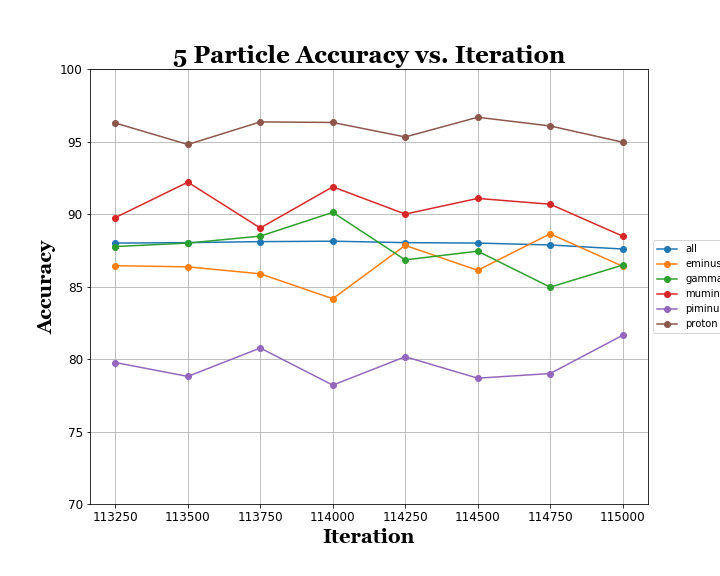
\includegraphics[width=0.3\textwidth]{../vgg16b/part5_vggb.png}\\
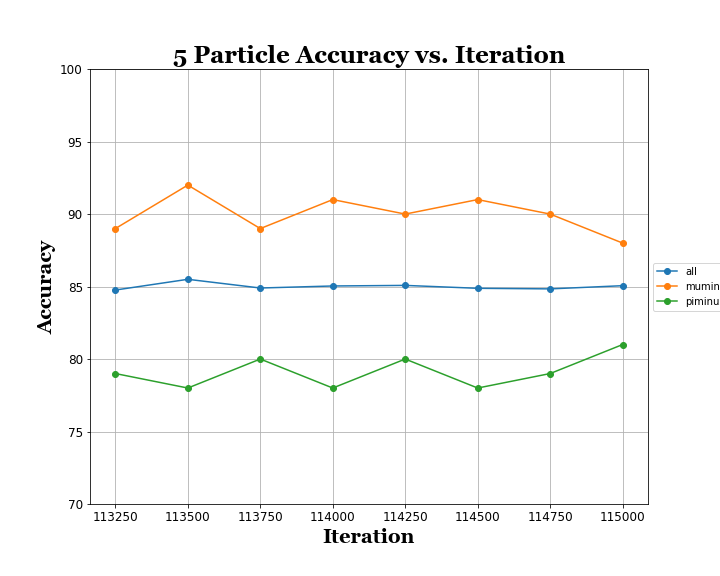
\includegraphics[width=0.3\textwidth]{../vgg16b/part_mu-pi_vggb.png}\\
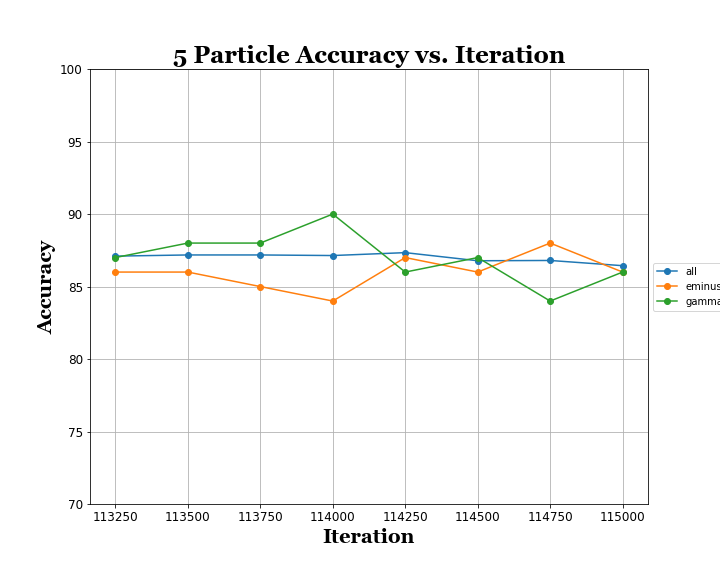
\includegraphics[width=0.3\textwidth]{../vgg16b/part_e-gamma_vggb.png}\\
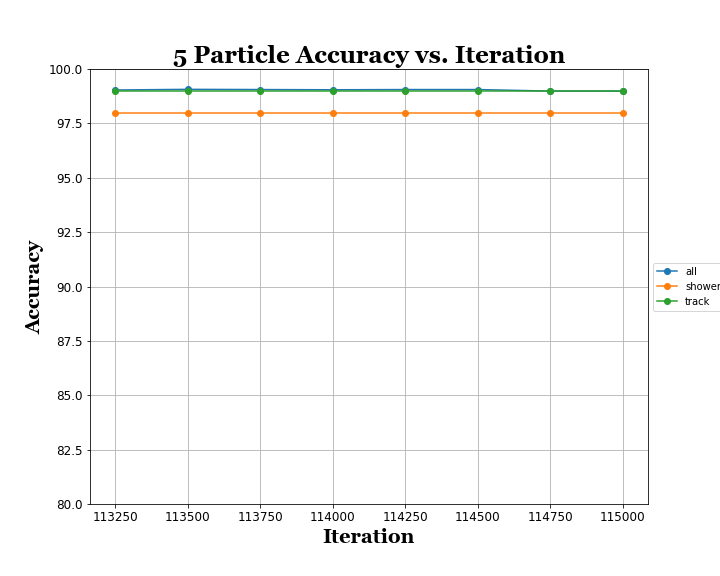
\includegraphics[width=0.3\textwidth]{../vgg16b/part_show-trk_vggb.png}
\caption{This is the (a) five particle classification, and (b) $\mu^-,\pi^-$, (c) $e,\gamma$, and (d) shower-track separations for the vgg16b network.}
  \label{fig:vgg16b}
\end{figure}


\subsection{vgg16c}



\section {Conclusions}

We have surveyed a variety of CNNs for the sake of classifying five charged particles as they appear in LArTPCs. Some interesting conclusions are that while Ref.~\cite{uB-JINST} achieved formidable performance, a few other networks do as well or better, and it is seen now that RestNetXYZ and VGG16XYZ are better choices.

We plan to start with these networks for future physics-identification tasks in MicroBooNE; we believe similar guidance for general TPCs applies there, as well. We advocate, per this study, that the full and infinite (hyper) parameter space for CNNs need not be explored in those future analyses in favor of the identified best-performing networks here.

%\appendix

%% Appendix 3: Bibliography %%
\newpage
%\section{Bibliography and References Cited}
%\bibliographystyle{JHEP}%{unsrt}
%\bibliography{arch}
\begin{thebibliography}{9}

\bibitem{AlexNet}
  Alex Krizhevsky {\it et al. },
  ``Imagenet Classification with Deep Convolutional Neural Networks,''
  \emph{NIPS} \textbf{25}, pages 1106–1114, 2012.

%MicroBooNE CNN JINST article \cite{ubooneCNN}
\bibitem{uB-JINST}
R. Acciarri {\it et. al.} [MicroBooNE collaboration],
"Convolutional Neural Networks Applied to Neutrino Events in a Liquid Argon Time Projection Chamber,"
\emph{1611.05531"} [phsics.ins-det].

\bibitem{SBN}
R. Acciarri {\it et al.} [SBN Collaboration],
``A Proposal for a Three Detector Short-Baseline Neutrino Oscillation Program in the Fermilab Booster Neutrino Beam,''
\emph{arXiv:1503.01520} [physics.ins-det].

\bibitem{DUNE}
R.~Acciarri {\it et al.} [DUNE Collaboration],
  ``Long-Baseline Neutrino Facility (LBNF) and Deep Underground Neutrino Experiment (DUNE) : Volume 1: The LBNF and DUNE Projects,''
  \emph{arXiv:1601.05471} [physics.ins-det].

\bibitem{dayabay}
E. Racah {\it et al.} ``Revealing Fundamental Physics from the Daya Bay Neutrino Experiment using Deep Neural Networks,'' \emph{arXiv:1601.07621}.

\bibitem{nova}
A. Aurisano {\it et al.}, ``A Convolutional Neural Network Neutrino Event Classifier,'' 2016 \emph{JINST} 11 P09001.

\bibitem{NEXT}
J.~Renner {\it et al.} [NEXT Collaboration],
``Background rejection in NEXT using deep neural networks,''
\emph{arxiv:1609.06202}.

\bibitem{larsoft050800}
LArSoft release {\it redmine} \textbf{05.08.00} \protect\url{https://cdcvs.fnal.gov/redmine/projects/larsoft/wiki/ReleaseNotes050800}.

\bibitem{uboonecode050800}
uboonecode release {\it redmine} \textbf{05.08.00} \protect\url{https://cdcvs.fnal.gov/redmine/projects/uboonecode/wiki/ReleaseNotes050800}.

\bibitem{LArCV}
 Genty, Terao and Wongjirad, LArCV: LArTPC Image Processing/Analysis Framework for Deep Learning \protect\url{https://www.github.com/LArbys/LArCV} %\protect\url{http://microboone-docdb.fnal.gov:8080/cgi-bin/ShowDocument?docid=5847}
 
\bibitem{caffe}
 Y. Jia {\it et al.}, ``Caffe: Convolutional Architecture for Fast Feature Embedding,'' {\emph arXiv:1408.5093}, 2014.
 
\bibitem{GoogLeNet}
Christian Szegedy {\it et al.}, ``Going Deeper with Convolutions,''
  \emph{arXiv:1409.4842}, 2014.

\bibitem{fasterrcnn}
Ren, Shaoqing and He, Kaiming and Girshick, Ross and Sun, Jian,
``Faster R-CNN: Towards Real-Time Object Detection with Region Proposal Networks,''
\emph{NIPS} \textbf{28} pages 91-99, 2015.

\bibitem{Inceptionv4}
Szegedy {\it et al.}, ``Inception-v4, Inception-ResNet and the Impact of Residual Connections on Learning,'' \emph{arXiv:1602.07261}.

\bibitem{ResNet}
  Kaiming He {\it et al.}, ``Deep Residual Learning for Image Recognition,'' \emph{arXiv:1512.03385}.

\bibitem{ROOT}
Rene Brun and Fons Rademakers,
``ROOT -- An object oriented data analysis framework,''
{\it NIM} {\bf A389} 81-86, 2015.

\bibitem{titanx}
NVIDIA GeForce Titan X GPU Card Specification, \protect\url{http://www.geforce.com/hardware/desktop-gpus/geforce-gtx-titan-x/specifications}

\bibitem{geant4}
S. Agostinelli {\it et al.}, ``GEANT4: A Simulation toolkit,''
{\it NIM} {\bf A506} 250-303, 2003.

\bibitem{ubnoisefiltering}
MicroBooNE Collaboration, ``TPC Noise Filtering,'' MicroBooNE Public Note 1016-PUB.
\protect\url{http://www-microboone.fnal.gov/publications/publicnotes/index.html}

\bibitem{ubsignalprocessing}
MicroBooNE Collaboration. ``TPC Signal Processing,'' MicroBooNE Public Note 1017-PUB.
\protect\url{http://www-microboone.fnal.gov/publications/publicnotes/index.html}

\bibitem{backprop}
Montavon {\it et al.}, ``Neural Networks: Tricks of the Trade,'' Springer 2012.

\bibitem{BNB}
A. A. Aguilar-Arevalo {\it et al.}, ``The Neutrino Flux Prediction at MiniBooNE,'' \emph{PRD} \textbf{78}, 072002, 2009

\bibitem{genie}
C. Andreopoulos {\it et al.}, ``The GENIE Neutrino Monte Carlo Generator,''
{it NIM} {\bf A614} 87-104, 2010.
  
\bibitem{BatchNorm}
  Ioffe {\it et al.}, ``Batch Normalization: Accelerating Deep Network Training by Reducing Internal Covariate Shift,'' Proc. of the 32nd Intl. Conf. on Machine Learning 37, 2015.

\bibitem{dropout}
  Srivastava  {\it et al.}, ``Dropout: A Simple Way to Prevent Neural Networks from Overfitting,'' Journal of Machine Learning Research 15 1929-1958, 2014.

\bibitem{alphago}
D. Silver {\it et al.}, ``Mastering the game of Go with deep neural networks and tree search,'' Nature 529, 484–489, 2016.

\bibitem{rmsprop}
Tieleman, Tijmen and Hinton, Geoffrey. ``Lecture 6.5-rmsprop: Divide the gradient by a running
average of its recent magnitude,'' COURSERA: Neural Networks for Machine Learning, 4, 2012.

\bibitem{ccnote}
  MicroBooNE Collaboration, ``Selection and kinematic properties of $\nu_\mu$ charged-current inclusive events in 5e19 POT of MicroBooNE data,''
  \protect\url{http://www-microboone.fnal.gov/publications/publicnotes/MICROBOONE-NOTE-1010-PUB.pdf}

\bibitem{stabilitytraining}
  Zheng {\it et al.}, ``Improving the Robustness of Deep Neural Networks via Stability Training,'' \emph{arXiv:1604.04326}.

\end{thebibliography}
\end{document}
